% ------------------------------------------------------------------------------------
\newpage
.
\newpage

{\color{lightgray} \hrule}
\begin{enumerate} \setcounter{enumi}{2}
	\item Implementar Random Walk Metropolis Hasting (RWMH) donde la distribución objetivo es $\mathcal{N}_2 (\mu, \Sigma)$, con
	\begin{equation} \label{eq:7}
		\mu = \binom{3}{5}, \quad \Sigma = \left(
		\begin{array}{cc}
			1 & 0.9 \\
			0.9 & 1
		\end{array} \right).
	\end{equation}
	Utilizar como propuesta $\varepsilon_t \sim \mathcal{N}_2 (0,\sigma I)$. ¿Cómo elegir $\sigma$ para que la cadena sea eficiente? ¿Qué consecuencias tiene la elección de $\sigma$?
	
	Como experimento, elige como punto inicial $x_0 = \binom{1000}{1}$ y comenta los resultados.
\end{enumerate}

Para todos los incisos del ejercicio anterior:
\begin{itemize}
	\item Establece cual es tu distribución inicial.
	\item Grafica la evolución de la cadena.
	\item Indica cuál es el Burn-in.
	\item Comenta qué tan eficiente es la cadena.
	\item Implementa el algoritmo MH considerando una propuesta diferente.
\end{itemize}

\textcolor{BrickRed}{\it Respuesta:}

En el archivo \textcolor{mediumblue}{ejercicio3\_tarea7.py} se implementan las funciones

\begin{itemize}
	\item \textit{contornos()}: grafica los contornos de la densidad (se muestran los contornos de la distribución real debajo y se sobrepone la cadena generada.
	\item \textit{marginal\_histograms()}: genera los histogramas de las cadenas marginales.
	\item \textit{plot\_evolution\_burn\_in()}: grafica la evolución de las cadenas de Markov marginales y sobrepone el burn-in calculado.
	\item \textit{moving\_average()}: calcula la media móvil.
	\item \textit{estimate\_burn\_in()}: Determinar cuándo se estabiliza la media móvil. Esta técnica consiste en observar la media móvil de las muestras y encontrar cuándo esta se estabiliza. Es una aproximación para el burn-in.
\end{itemize}

Luego, se define la función \textit{RANDOM\_WALK\_METROPOLIS\_HASTINGS()} la cual implementa algoritmo Random Walk Metropolis-Hastings en $\mathbb{R}^n$. Toma como argumentos:
\begin{itemize}
	\item La función objetivo $f$ (en este caso es \eqref{eq:7}).
	\item El valor inicial $x_0$.
	\item La matriz de covarianza (en este caso es $\sigma I$).
	\item El número de iteraciones del algoritmo (casi siempre se usa $N = 10,000$).
\end{itemize}

Regresa la cadena de Markov simulada en $\mathbb{R}^n$ y usa el criterio de aceptación: si $y_t$ es la propuesta dada por $y_t = x_t + \varepsilon_t$ en $x_t$, entonces se acepta $y_t$ con probabilidad $\rho(x_t, y_t)$ con
\begin{equation}
	\rho(x,y) = \min\left\{1, \frac{f(y)}{f(x)} \right\}
\end{equation}
y se rechaza con probabilidad $1-\rho(x_t, y_t)$. Luego, se define la función \textit{f\_pdf()} la cual implementa \eqref{eq:7}.

Finalmente, se simulan $4$ cadenas de Markov en $\mathbb{R}^2$ con diferentes puntos iniciales y matrices de covarianza para la propuesta. Se grafican los contornos de la densidad y la evolución de la cadena de Markov en $\mathbb{R}^2$, los histogramas marginales y la evolución de las cadenas de Markov
marginales con el burn-in estimado.

% --------------------------------------------------------------------------------
\textbf{Ejemplo 1:} Se usó el punto inicial $x_0=(1,1)$, y $\sigma = 1$, i.e., la matriz de covarianzas fue $I$ y se obtuvieron los siguientes resultados:

Tasa de aceptación: $31.10\%$, burn-in estimado: $133$ iteraciones, promedio de la cadena: $[2.948, 4.944]$ y covarianza de la cadena: $\binom{1.016\quad0.911}{0.911\quad1.007}$. El algoritmo fue eficiente debido a la similitud en la magitud de $\sigma$ respecto a la lejanía de $x_0$ de $(3,5)$.
\begin{figure}[h!]
	\centering
	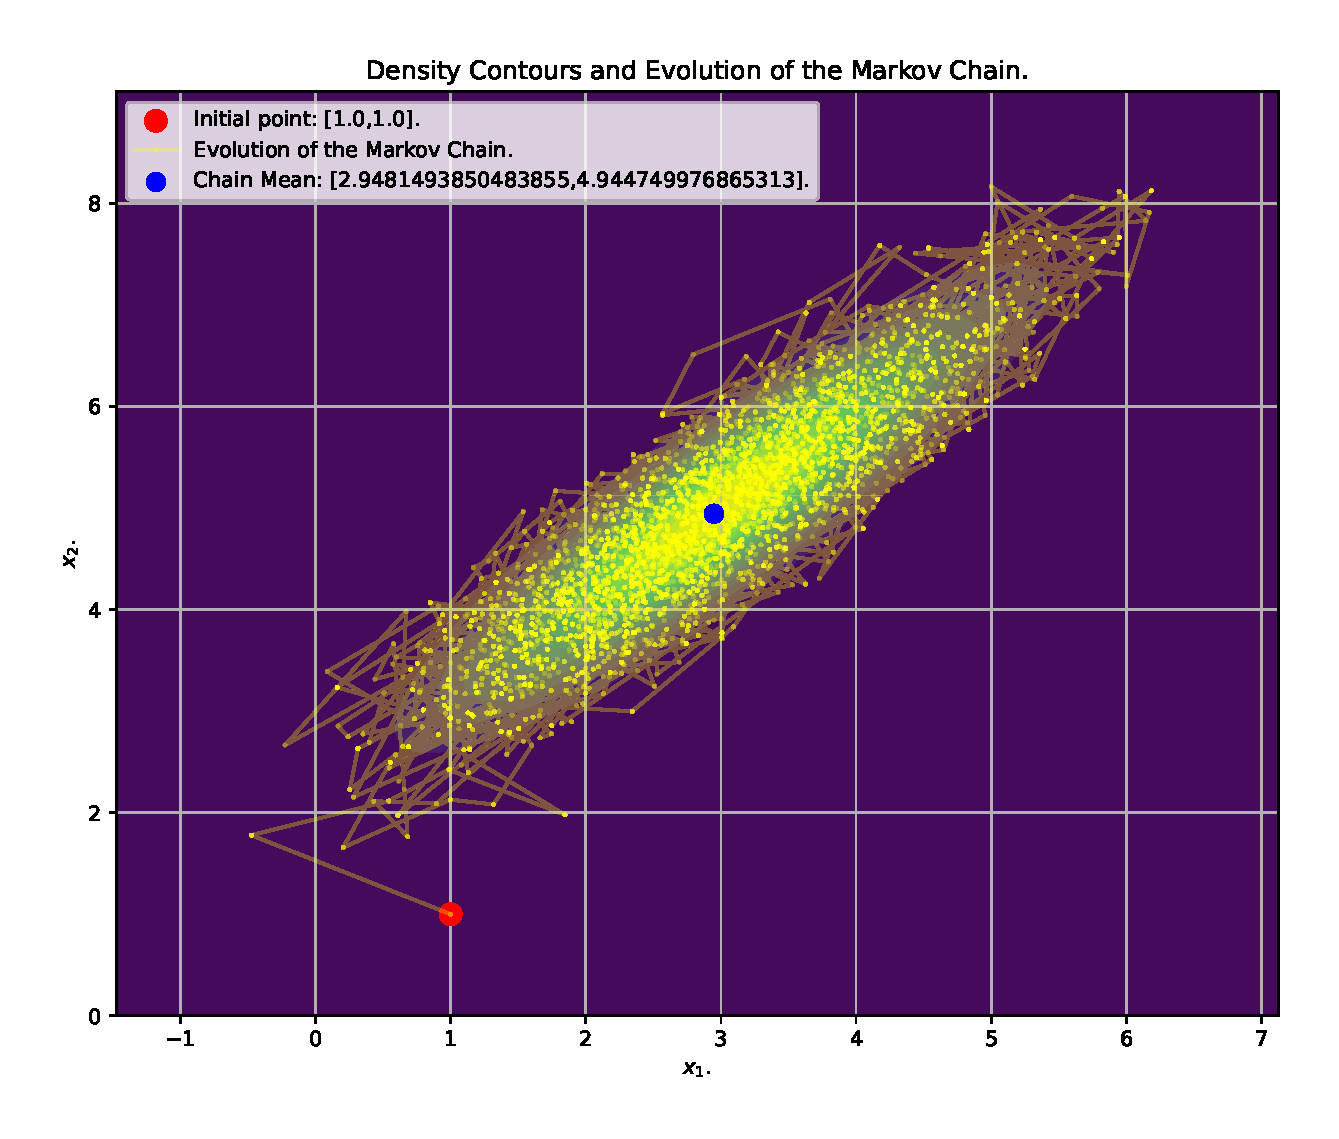
\includegraphics[width=0.84\textwidth]{IMAGENES/ex3/contour_example1.pdf}
\end{figure}
\begin{figure}[h!]
	\centering
	\begin{minipage}{0.495\textwidth}
		\centering
		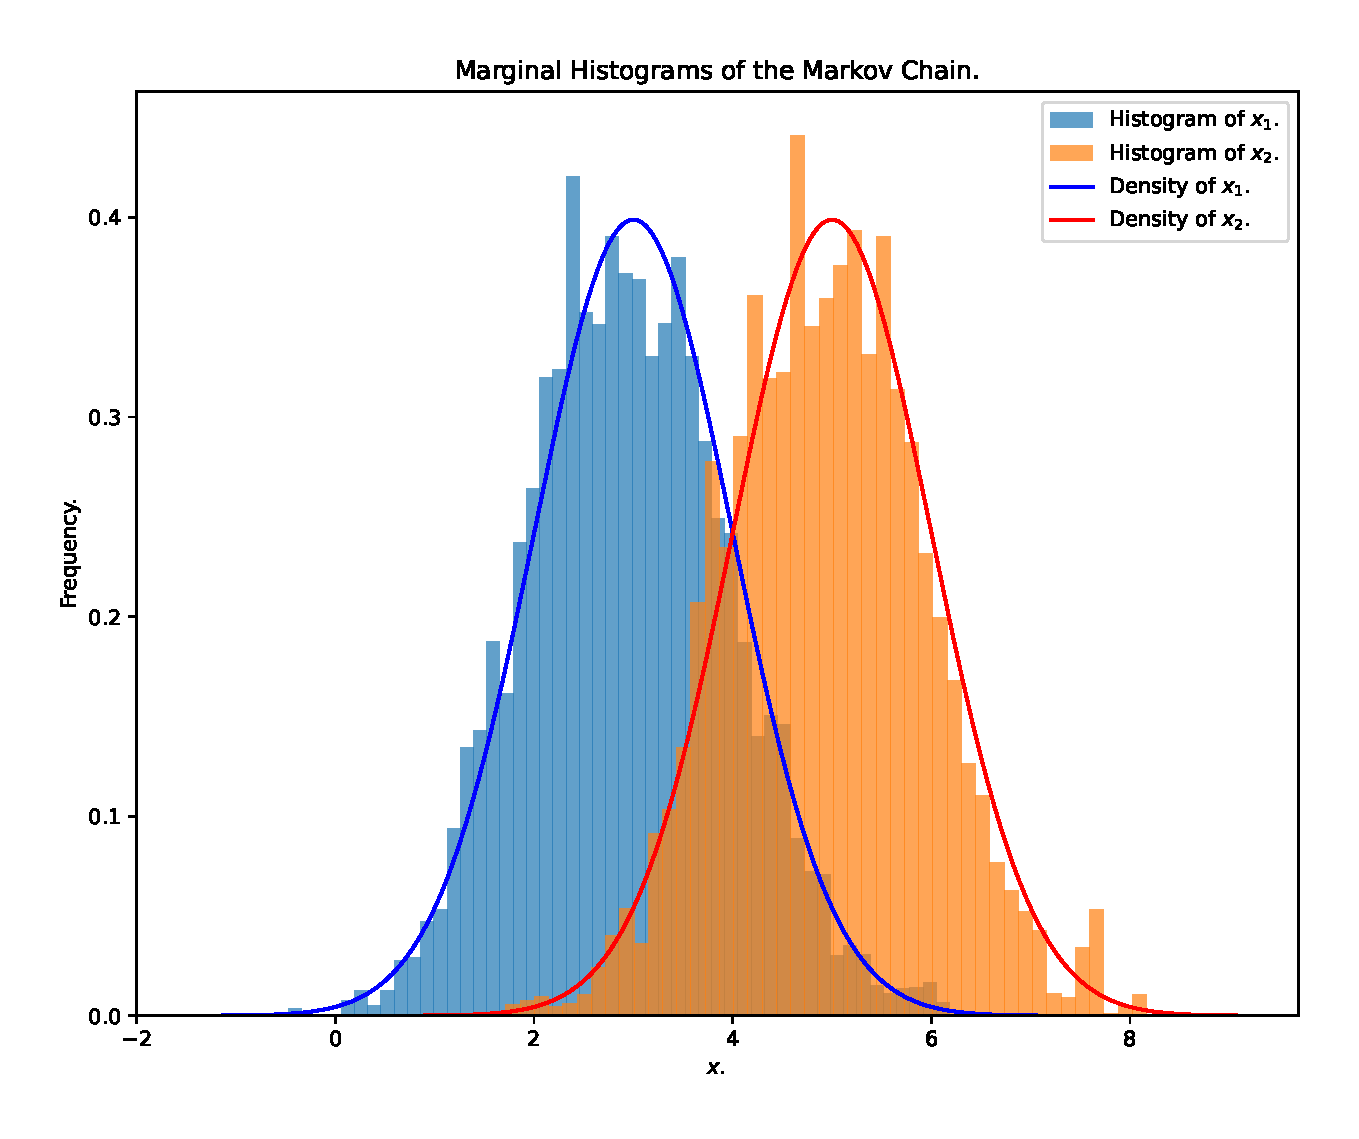
\includegraphics[width=\textwidth]{IMAGENES/ex3/histograms_example1.pdf}
	\end{minipage}
	\hfill
	\begin{minipage}{0.495\textwidth}
		\centering
		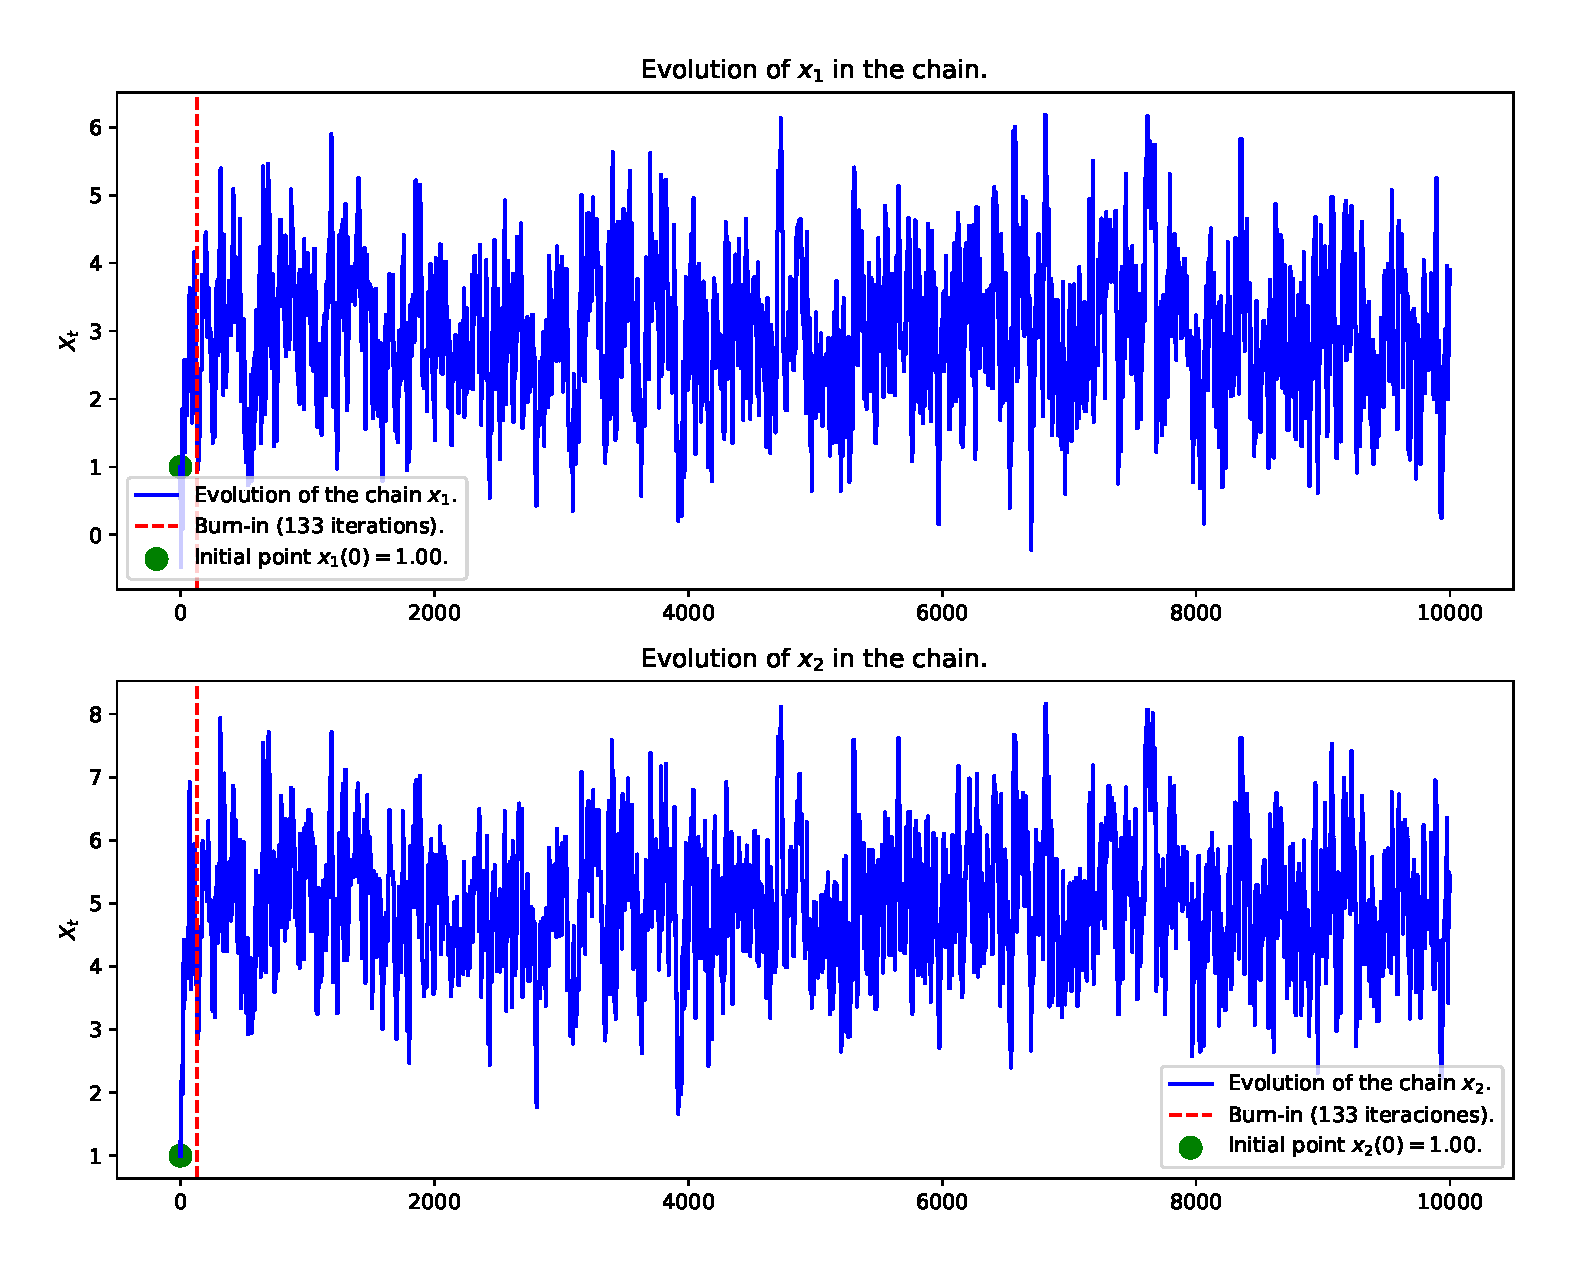
\includegraphics[width=\textwidth]{IMAGENES/ex3/evolution_example1.pdf}
	\end{minipage}
\end{figure}

% --------------------------------------------------------------------------------
\textbf{Ejemplo 2:} Se usó el punto inicial $x_0=(20,15)$, y se usó $\sigma = 20$, i.e., la matriz de covarianzas fue $20 I$ y se obtuvieron los siguientes resultados:

Tasa de aceptación: $4.06\%$, burn-in estimado: $263$ iteraciones, promedio de la cadena: $[2.931, 4.954]$ y covarianza de la cadena: $\binom{1.282\quad1.163}{1.163\quad1.266}$. El algoritmo fue eficiente debido a la similitud en la magitud de $\sigma$ respecto a la lejanía de $x_0$ de $(3,5)$.
\begin{figure}[h!]
	\centering
	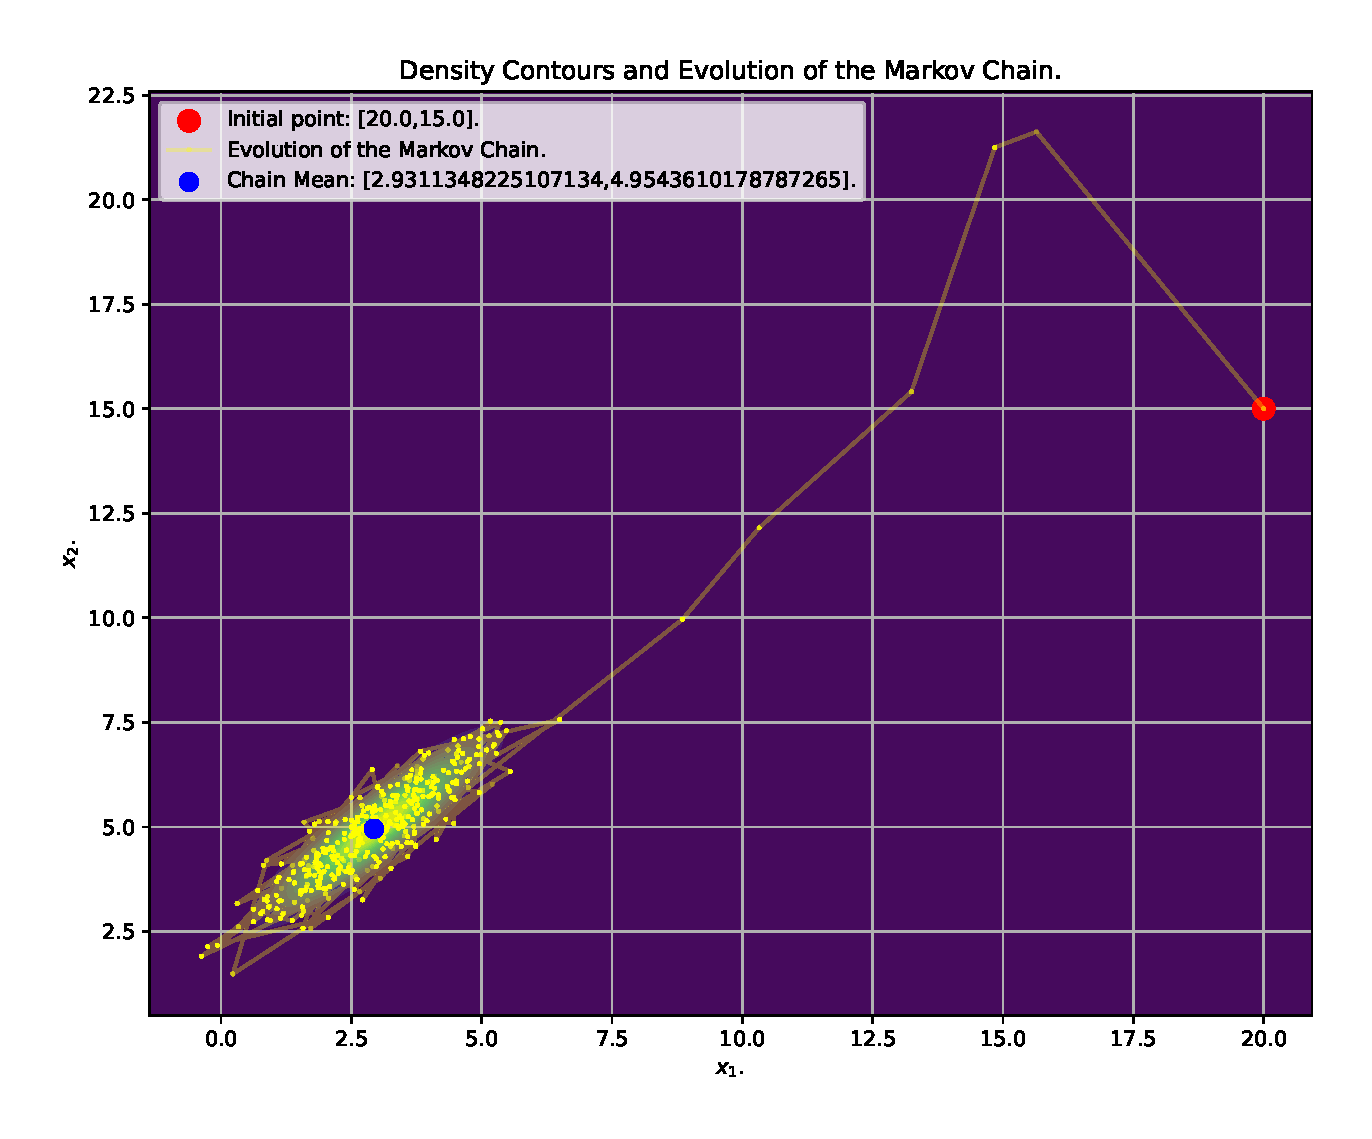
\includegraphics[width=0.87\textwidth]{IMAGENES/ex3/contour_example2.pdf}
\end{figure}
\begin{figure}[h!]
	\centering
	\begin{minipage}{0.495\textwidth}
		\centering
		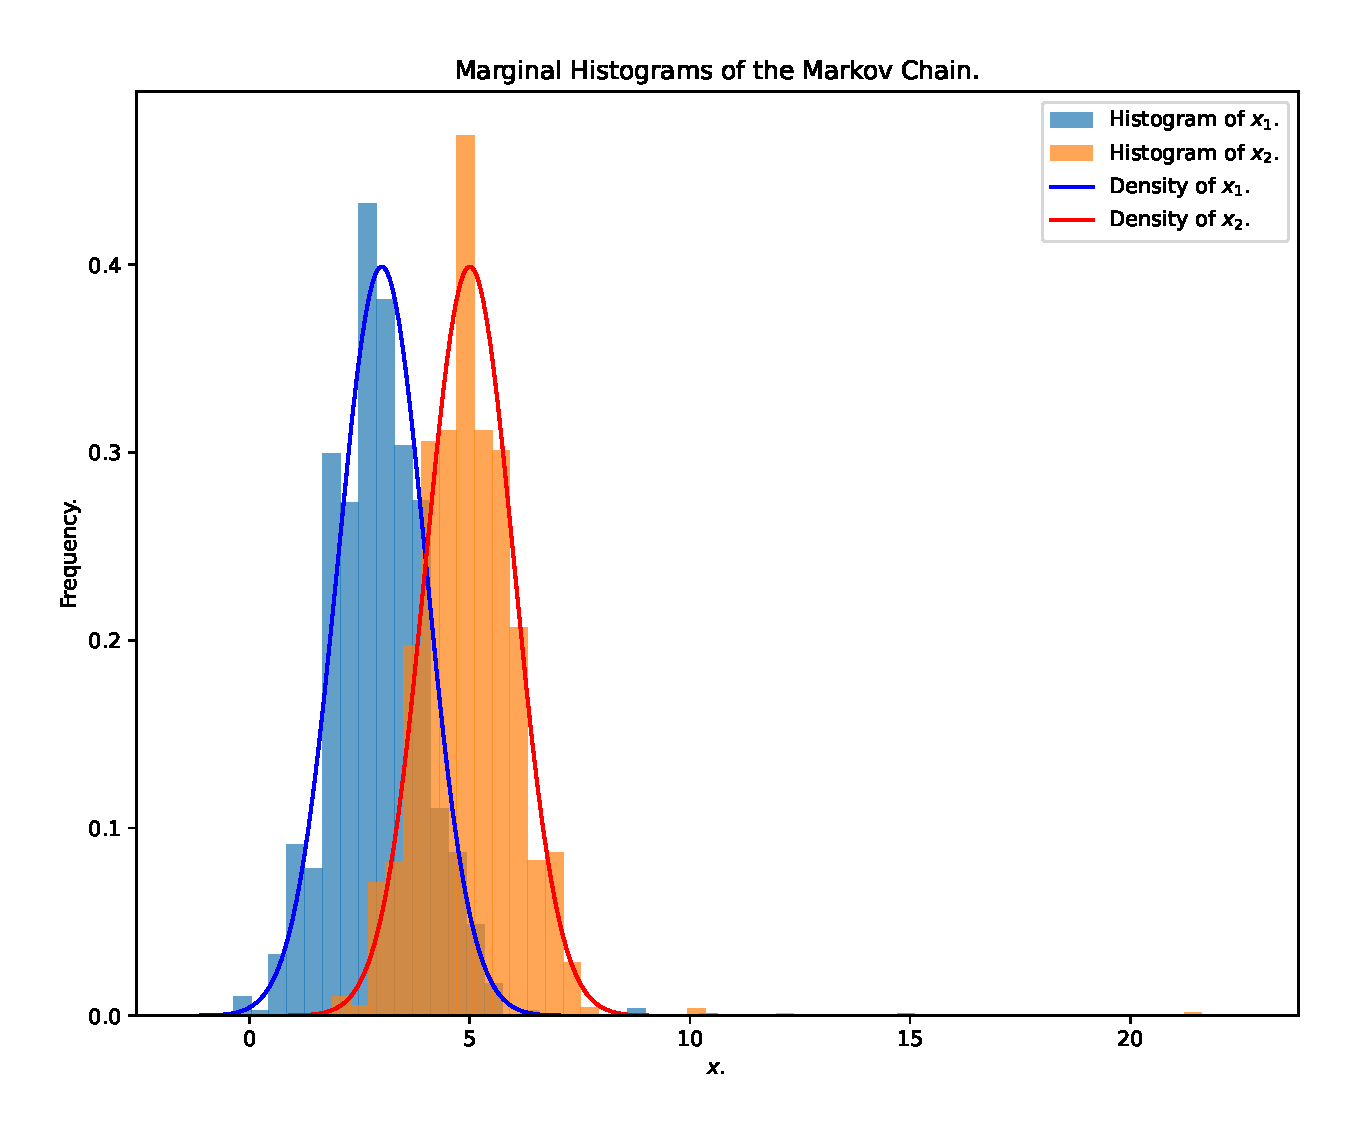
\includegraphics[width=\textwidth]{IMAGENES/ex3/histograms_example2.pdf}
	\end{minipage}
	\hfill
	\begin{minipage}{0.495\textwidth}
		\centering
		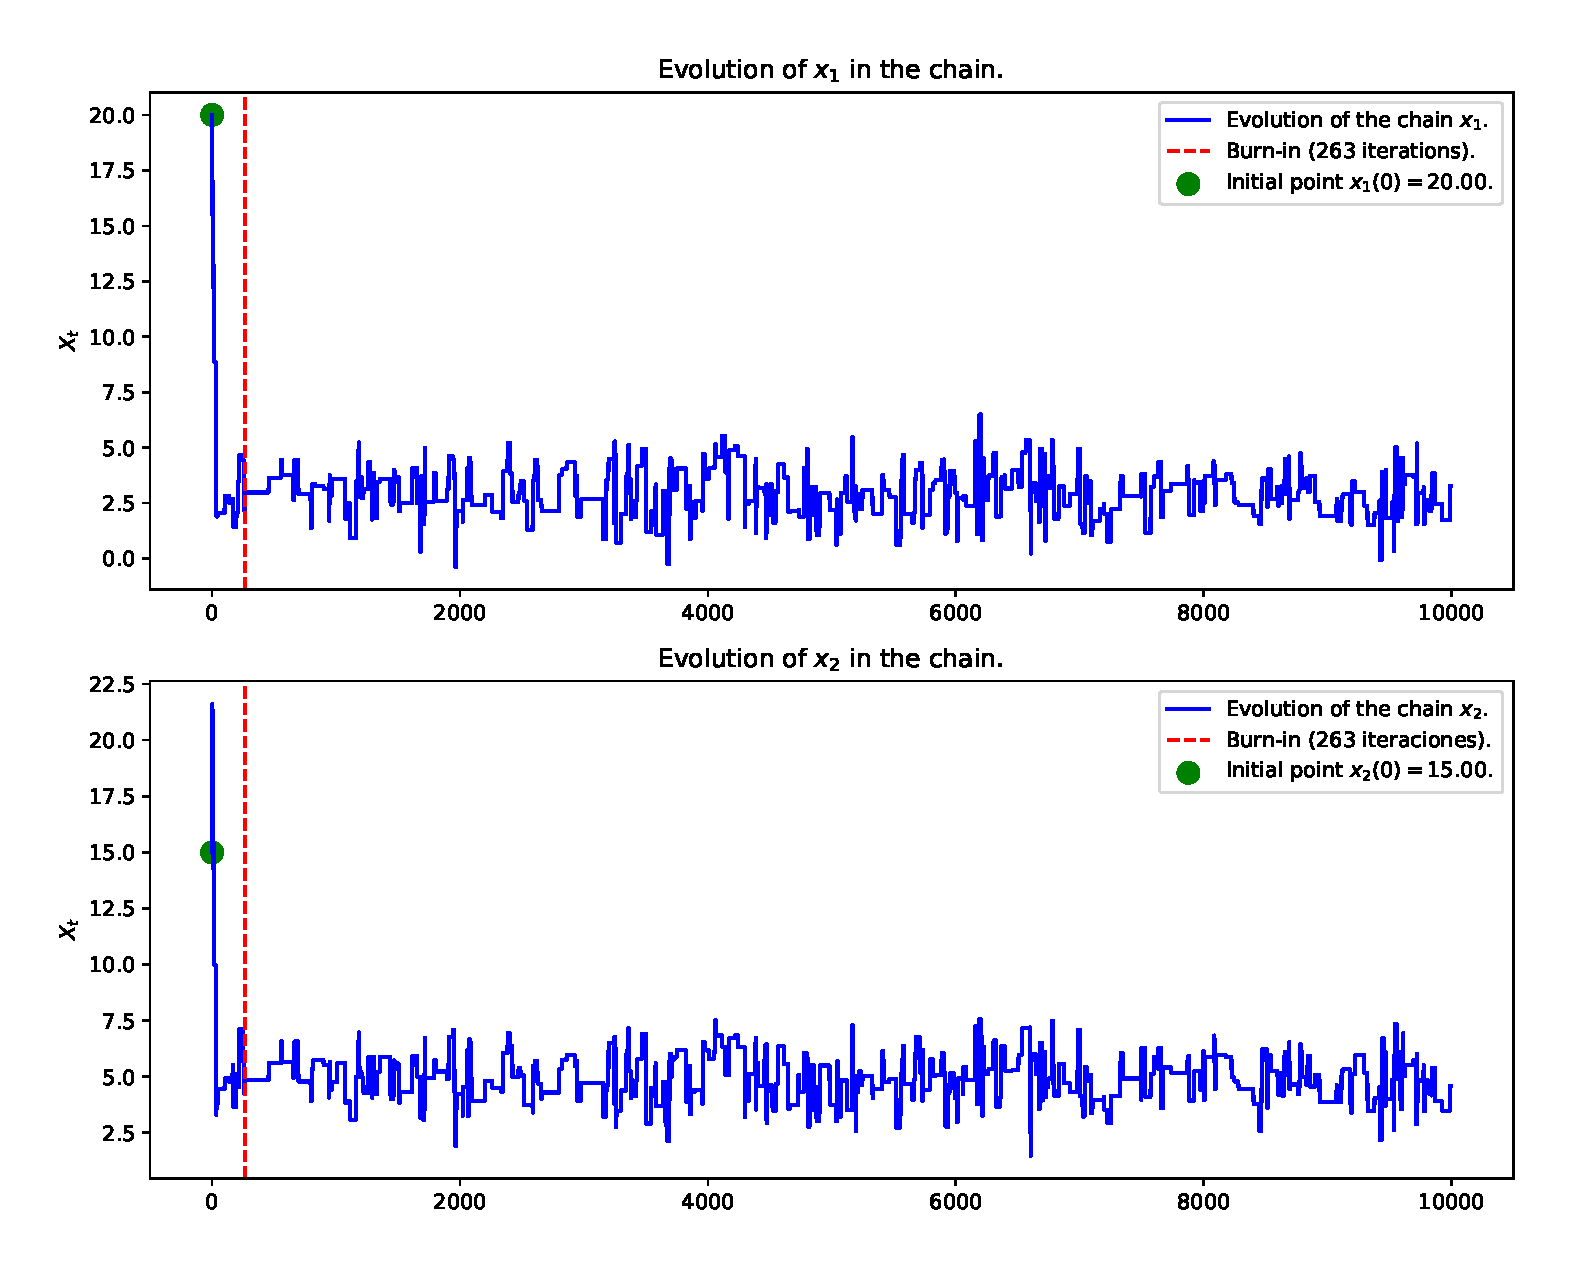
\includegraphics[width=\textwidth]{IMAGENES/ex3/evolution_example2.pdf}
	\end{minipage}
\end{figure}

% --------------------------------------------------------------------------------
\textbf{Ejemplo 3:} Se usó el punto inicial $x_0=(-20,-10)$, y se usó $\sigma = 25$, i.e., la matriz de covarianzas fue $25 I$ y se obtuvieron los siguientes resultados:

Tasa de aceptación: $4.05\%$, burn-in estimado: $162$ iteraciones, promedio de la cadena: $[2.851, 4.911]$ y covarianza de la cadena: $\binom{1.281\quad1.113}{1.113\quad1.147}$. El algoritmo fue eficiente debido a la similitud en la magitud de $\sigma$ respecto a la lejanía de $x_0$ de $(3,5)$.
\begin{figure}[h!]
	\centering
	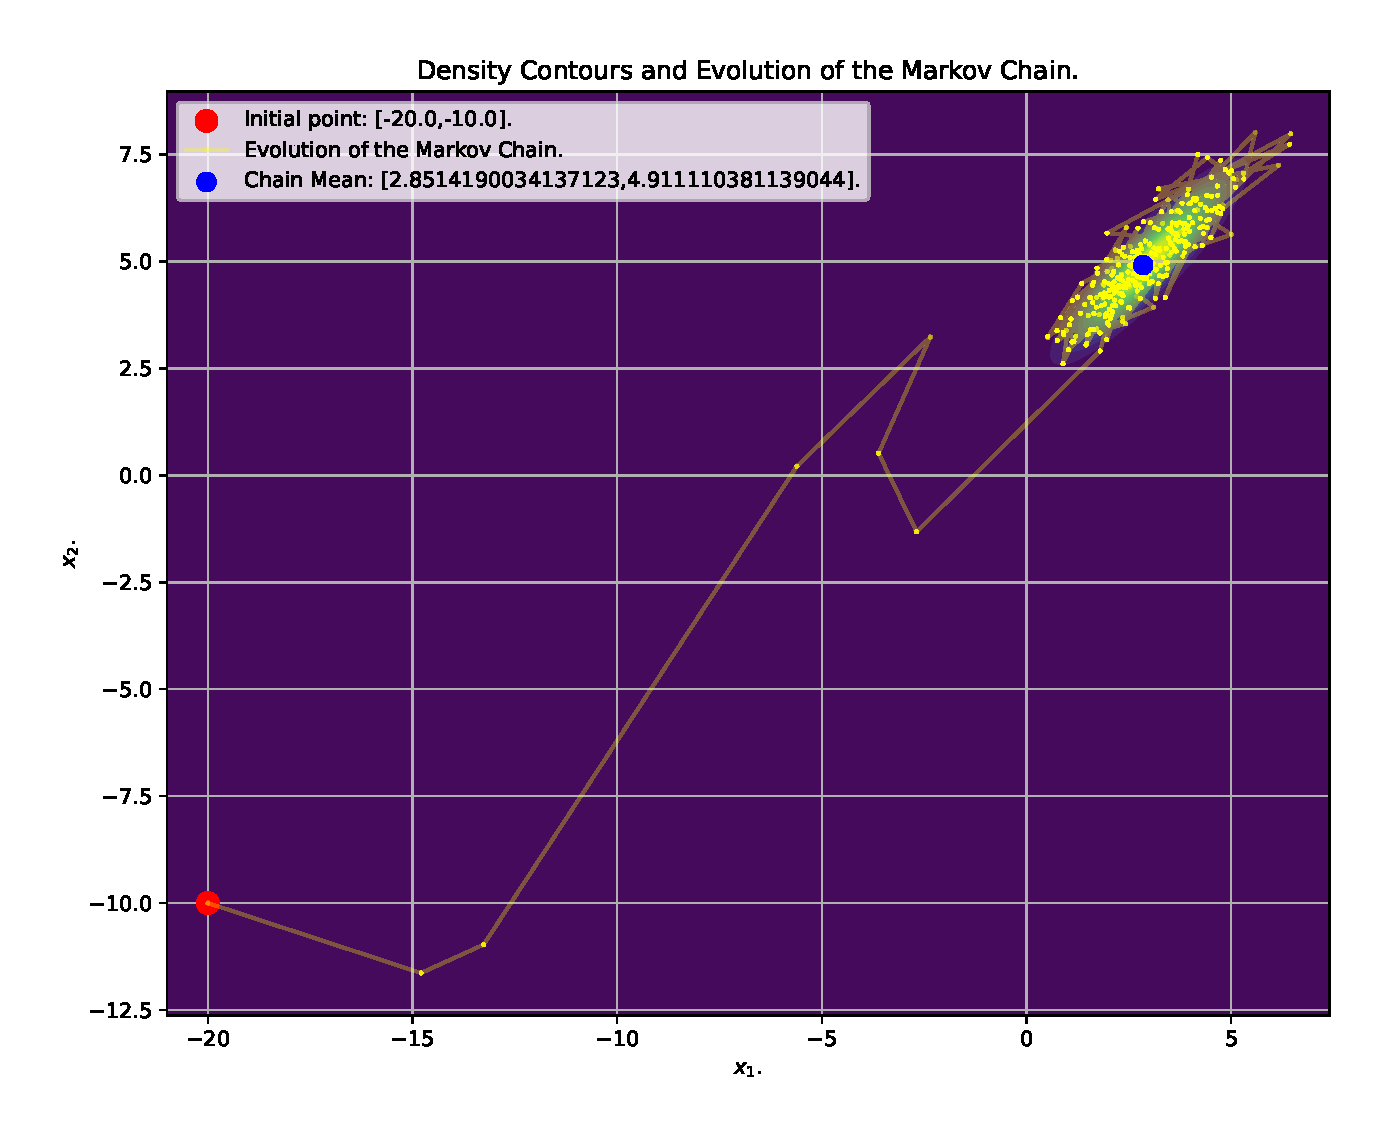
\includegraphics[width=0.87\textwidth]{IMAGENES/ex3/contour_example3.pdf}
\end{figure}
\begin{figure}[h!]
	\centering
	\begin{minipage}{0.495\textwidth}
		\centering
		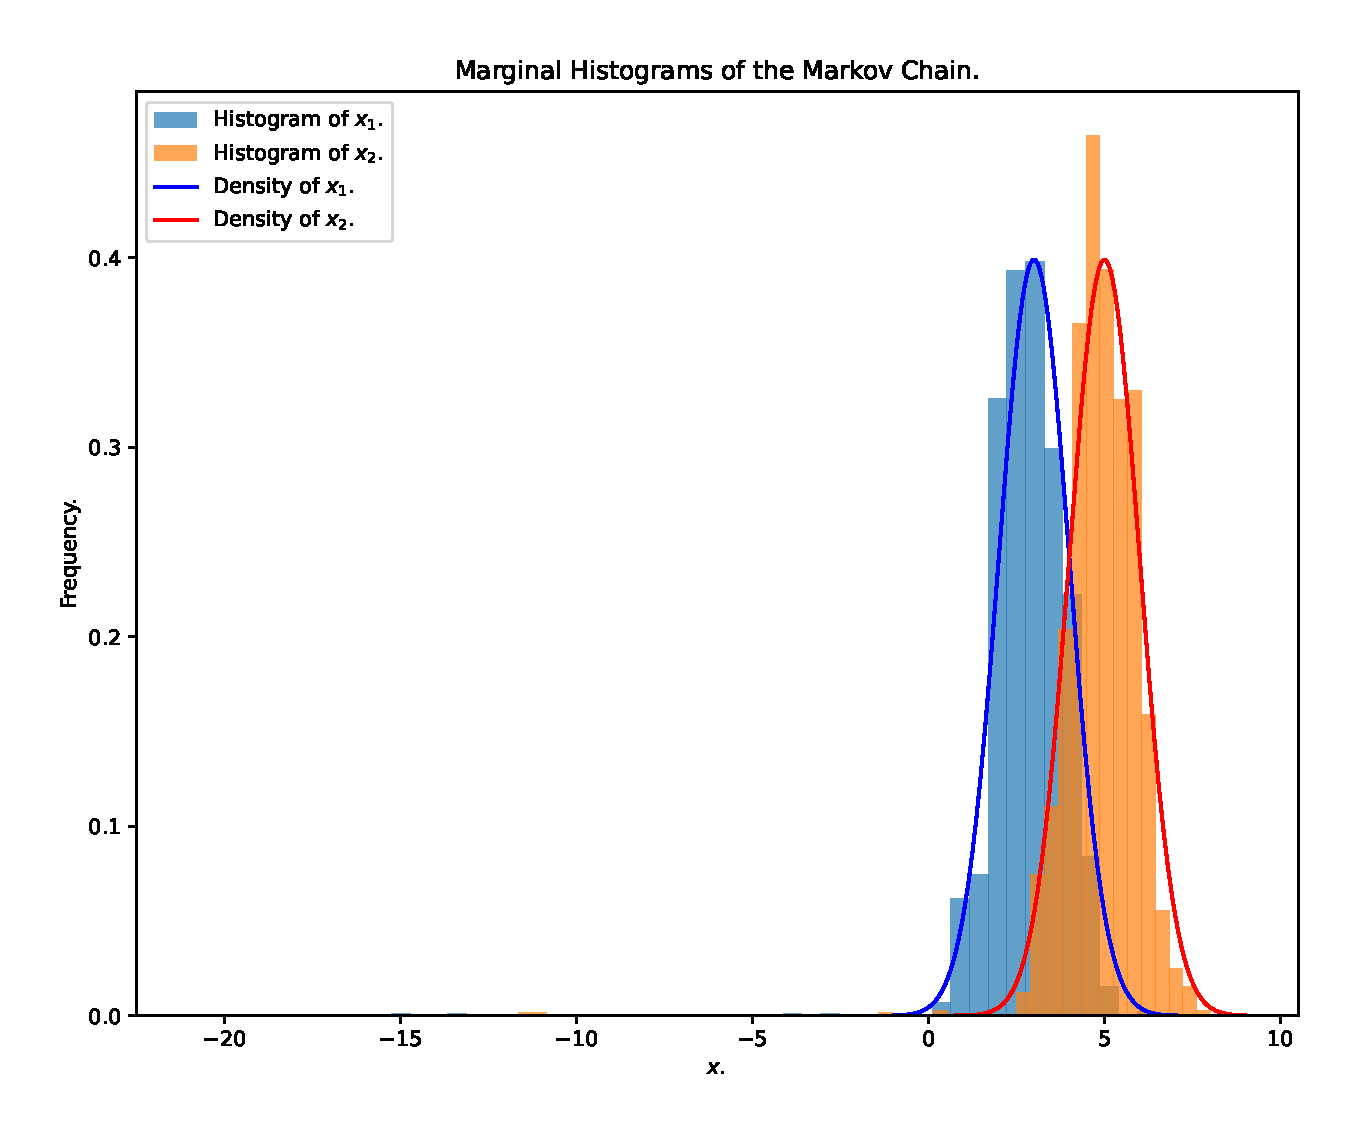
\includegraphics[width=\textwidth]{IMAGENES/ex3/histograms_example3.pdf}
	\end{minipage}
	\hfill
	\begin{minipage}{0.495\textwidth}
		\centering
		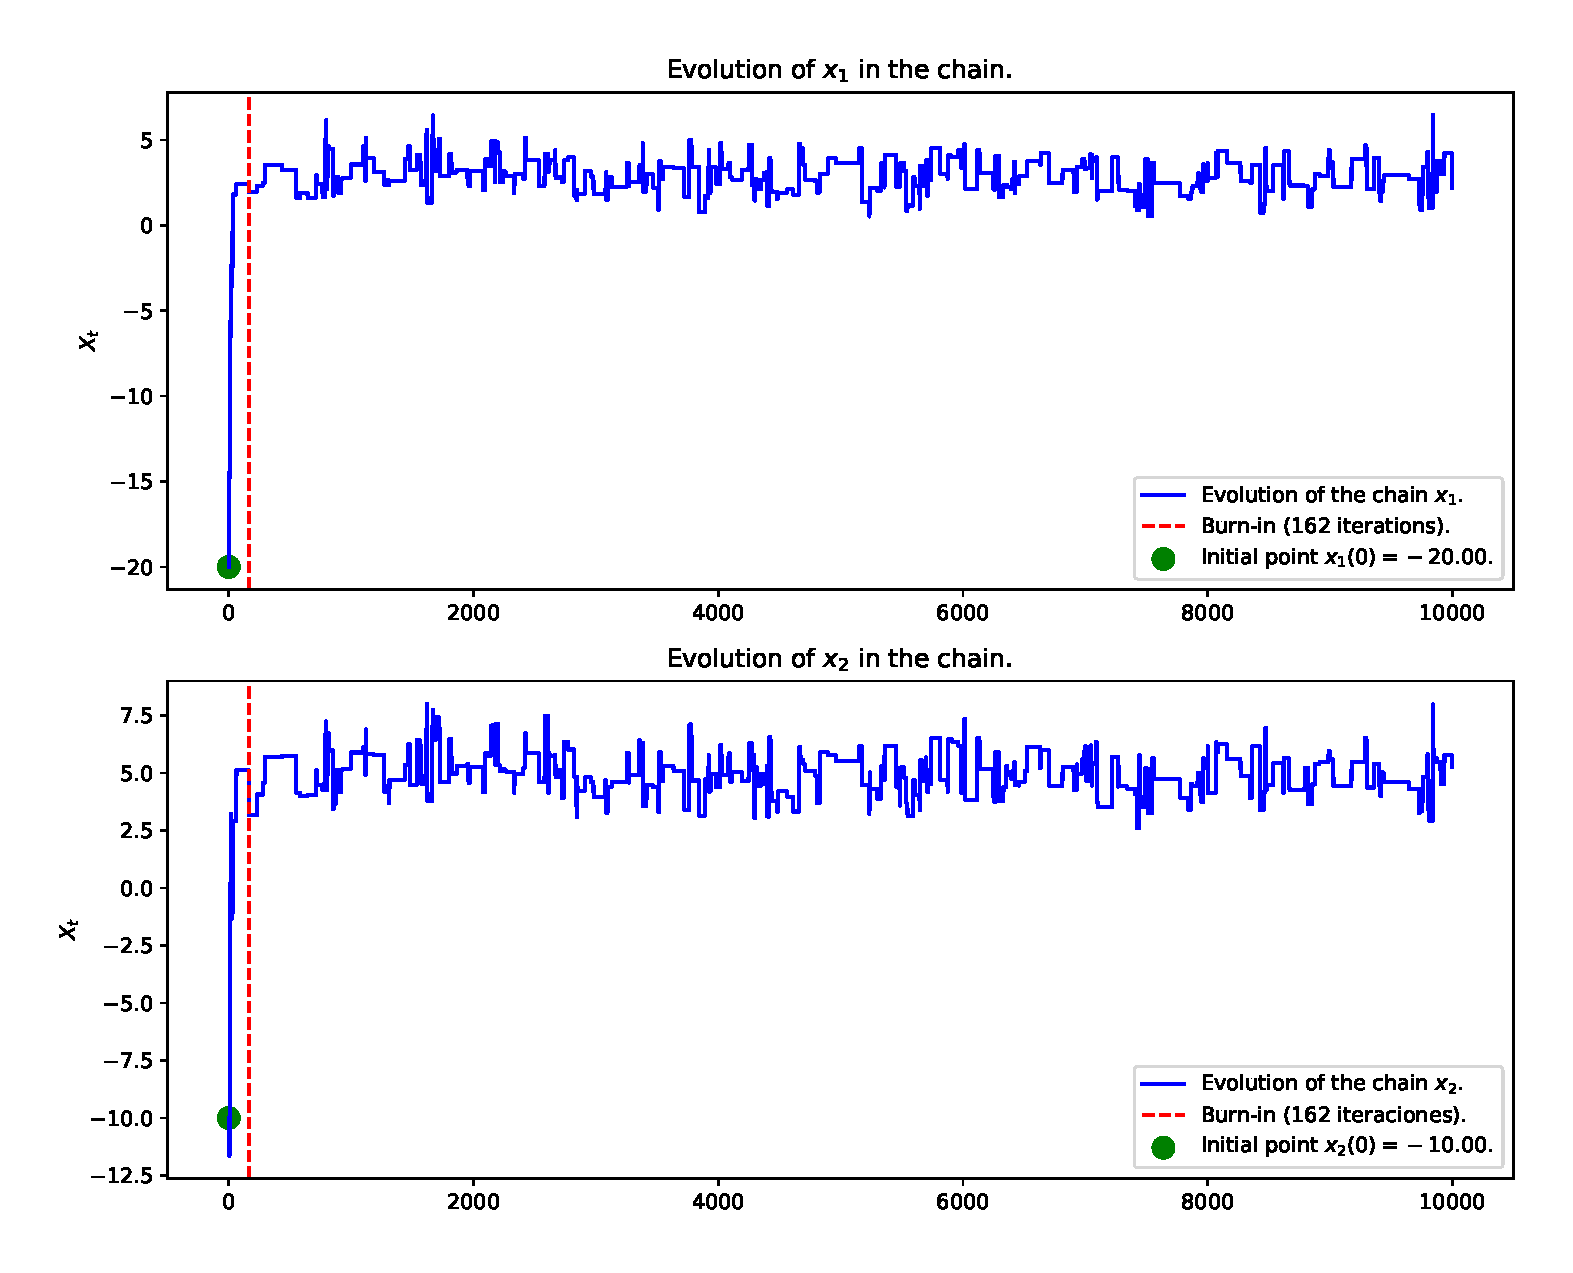
\includegraphics[width=\textwidth]{IMAGENES/ex3/evolution_example3.pdf}
	\end{minipage}
\end{figure}

% --------------------------------------------------------------------------------
\textbf{Ejemplo 4:} Se usó el punto inicial $x_0=(1000,1)$, y se usó $\sigma = 100$, i.e., la matriz de covarianzas fue $100 I$ y se obtuvieron los siguientes resultados:

Tasa de aceptación: $99.99\%$, burn-in estimado: $271$ iteraciones, promedio de la cadena: $[981.137, 1257.851]$ y covarianza de la cadena: $\binom{110724.962\quad37422.424}{37422.424\quad613530.619}$. El algoritmo no fue eficiente para ninguna configuración de parámetros debido a la lejanía de $x_0$ de $(3,5)$.
\begin{figure}[h!]
	\centering
	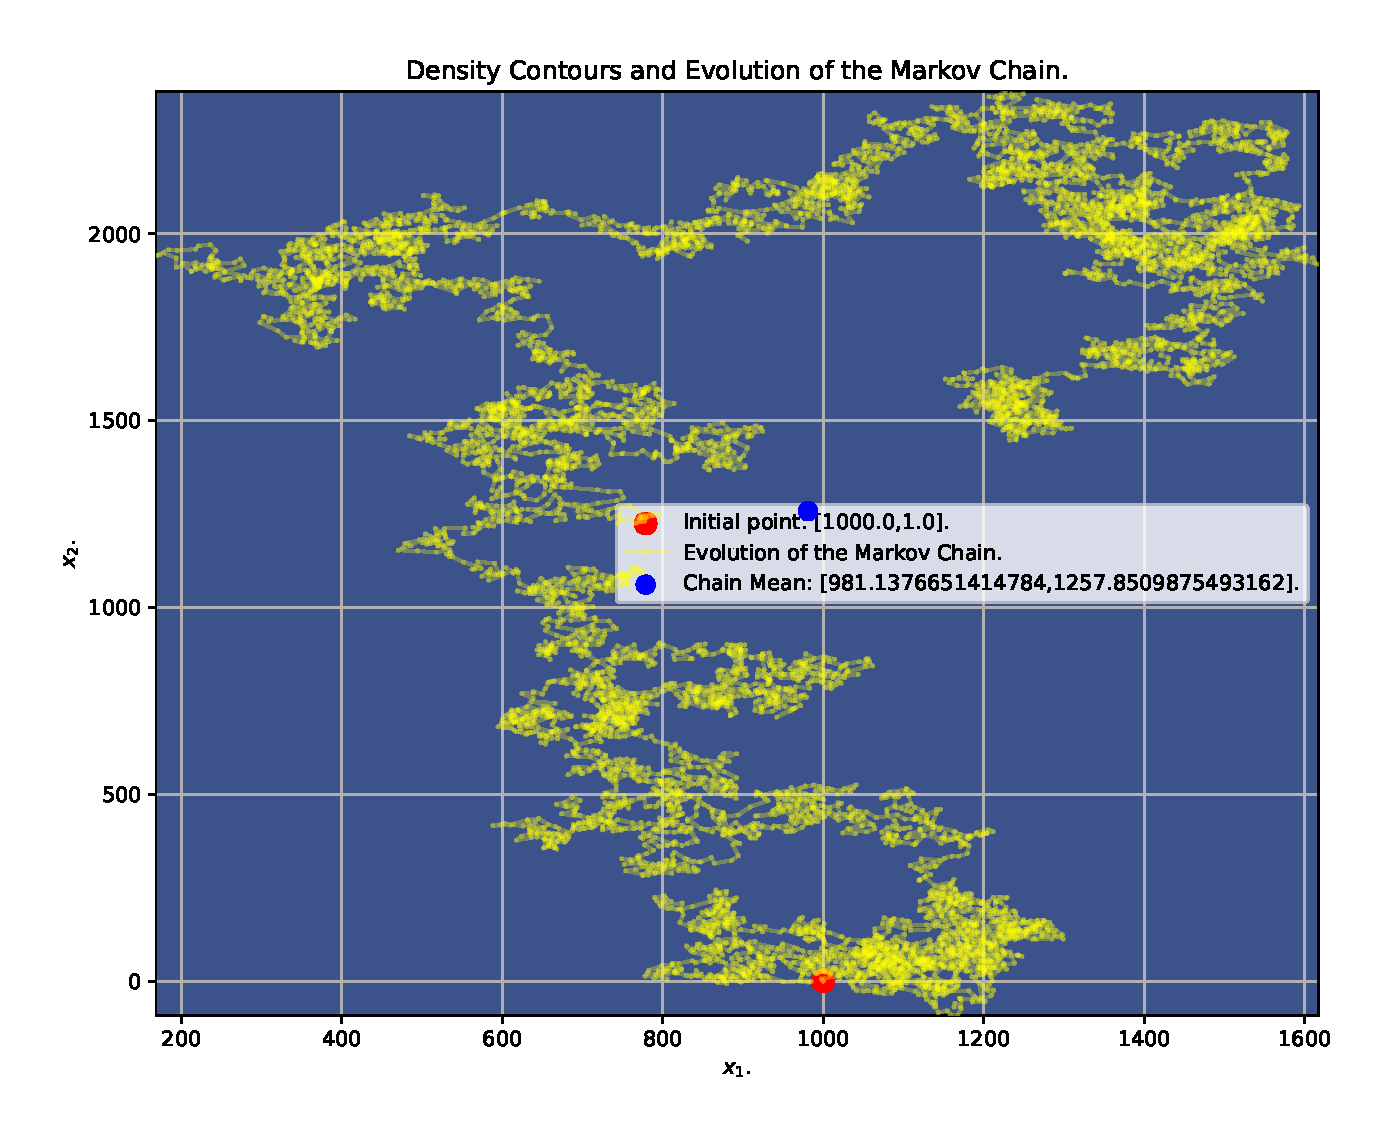
\includegraphics[width=0.87\textwidth]{IMAGENES/ex3/contour_example4.pdf}
\end{figure}

\begin{figure}[h!]
	\centering
	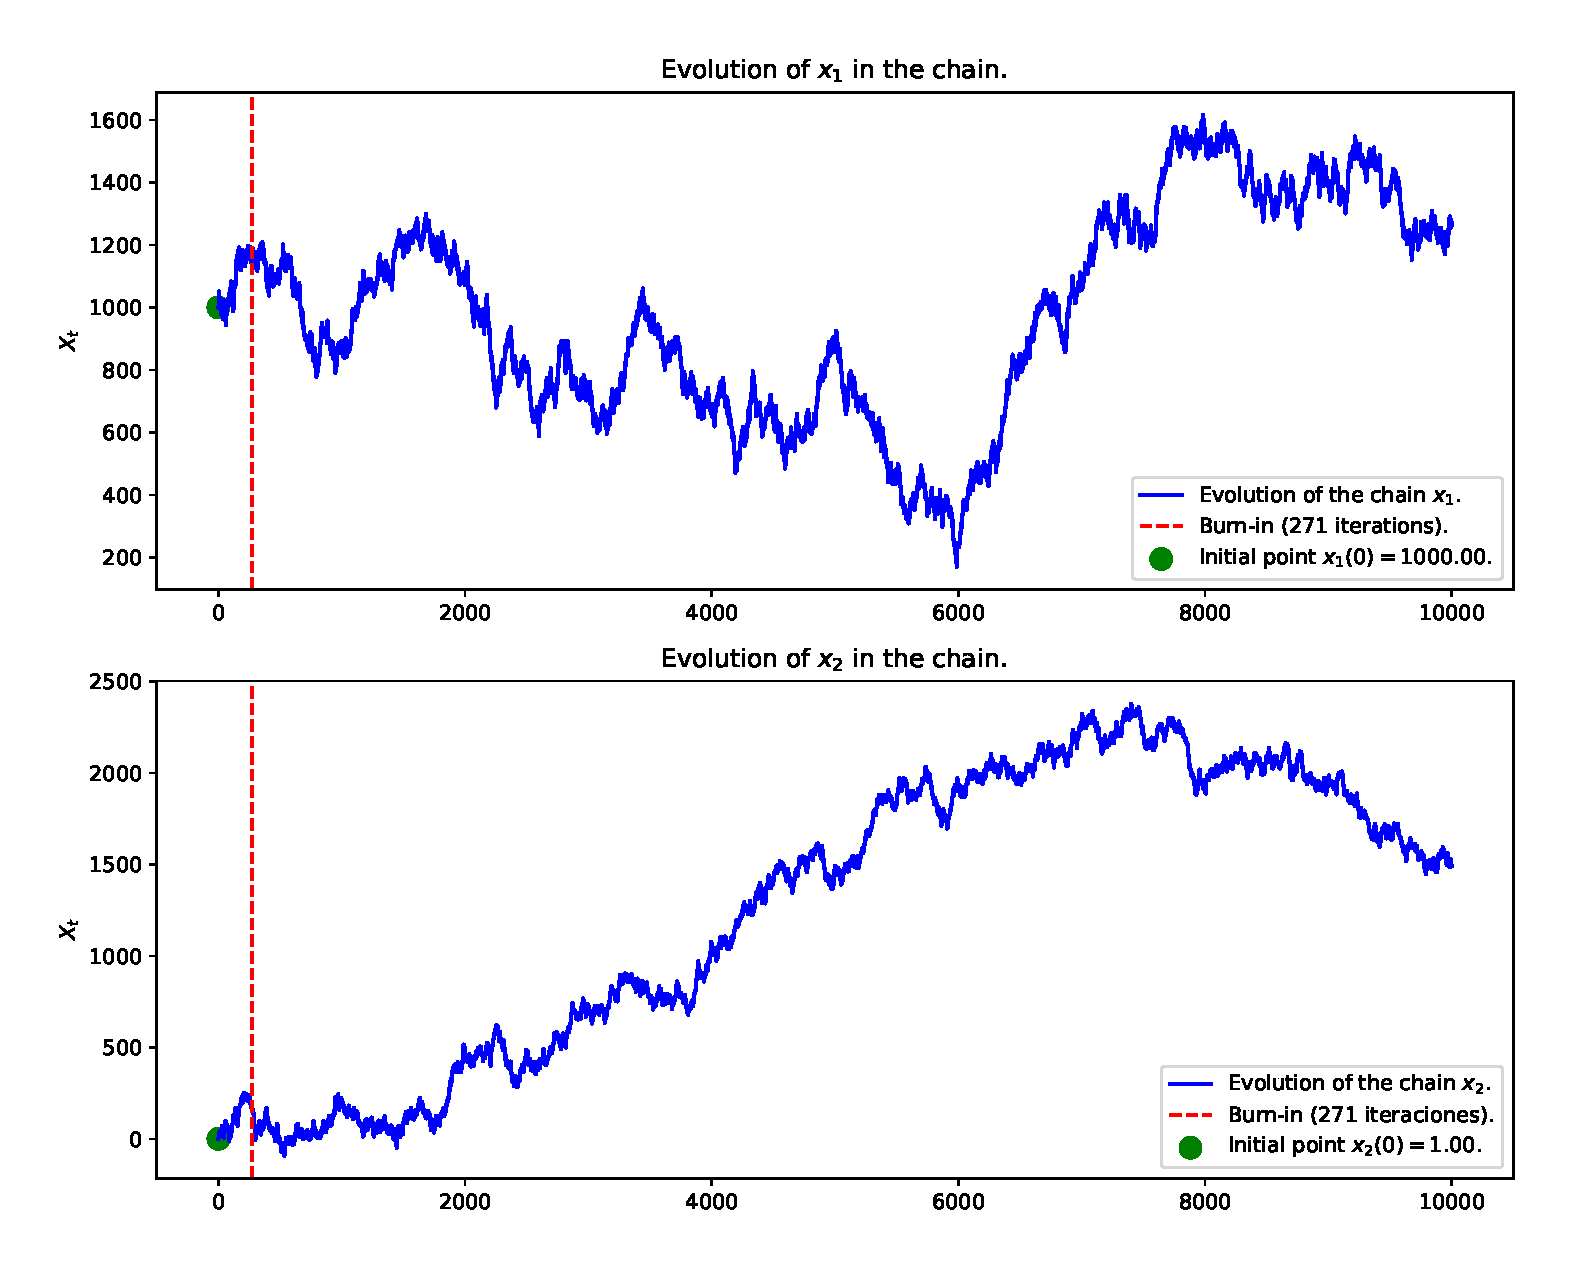
\includegraphics[width=0.8\textwidth]{IMAGENES/ex3/evolution_example4.pdf}
\end{figure}

\textbf{Comentarios finales:}

Mientras se revisaban diversos ejemplos variando parámetros como $\sigma$ y el punto inicial $x_0$, iba resultando que, según que tan lejos eligiéramos $x_0$ del punto $(3,5)$, iba a necesitar mayor varianza o un número mayor de iteraciones para que la cadena se encontrara cerca de $(3,5)$. El parámetro $\sigma$ controla el tamaño de los pasos en el proceso de Metropolis-Hastings. Se notó que las diferentes consecuencias de elegir diferentes valores de $\sigma$ son las siguientes:

\begin{itemize}
	\item $\sigma$ muy pequeño: Las propuestas estarán muy cerca del valor anterior, lo que puede resultar en una tasa de aceptación muy alta, pero la cadena se moverá muy lentamente por el espacio de estados, lo que lleva a una mayor correlación entre las muestras (un ejemplo de esto es el ejemplo $1$). En este caso, se necesitarán más iteraciones para cubrir toda la distribución objetivo, y el burn-in  será más largo.
	
	\item $\sigma$ muy grande: Las propuestas serán más lejanas, lo que puede llevar a una baja tasa de aceptación, ya que muchas propuestas serán rechazadas (ejemplos de esto son los ejemplos $2$ y $3$). La cadena puede quedarse atrapada en ciertas regiones, y será difícil explorar completamente el espacio de estados. Aquí también el burn-in puede será más largo, ya que la cadena podría tardar en estabilizarse.
\end{itemize}

Respecto a el punto inicial $x_0 = (1000,1)$ (se tiene un ejemplo en el ejemplo $4$), como se encontraba demasiado lejos de la zona donde se concentra el soporte de la distribución objetivo, generaba demasiados errores e indeterminaciones al momento de aplicar Metropolis-Hastings (específicamente al calcular la tasa de aceptación $\frac{f(y)}{f(x)}$). Los ''mejores'' resultados se tenían al usar varianzas muy grandes, sin embargo, en ninguno de los casos se logró la convergencia (no se logró la eficiencia). Esto se debe a que la probabilidad de este $x_0$ bajo la distribución objetivo es $0$, debido a su lejanía del punto $(3,5)$.


